
\subsection{Principio del palomar o Principio de Dirichlet}

El principio del palomar, también llamado principio de Dirichlet o principio de
las cajas, establece que si $n$ palomas se distribuyen en $m$ palomares, y si $n
> m$, entonces al menos habrá un palomar con más de una paloma. Otra forma de
decirlo es que $m$ huecos pueden albergar como mucho $m$ objetos si cada uno de
los objetos está en un hueco distinto, así que el hecho de añadir otro objeto
fuerza a volver a utilizar alguno de los huecos, como se observa en la Fig.
(\ref{palomar}). A manera de ejemplo: si se toman trece personas, al menos dos
habrán nacido el mismo mes.

\begin{figure}[h]
	\centering
	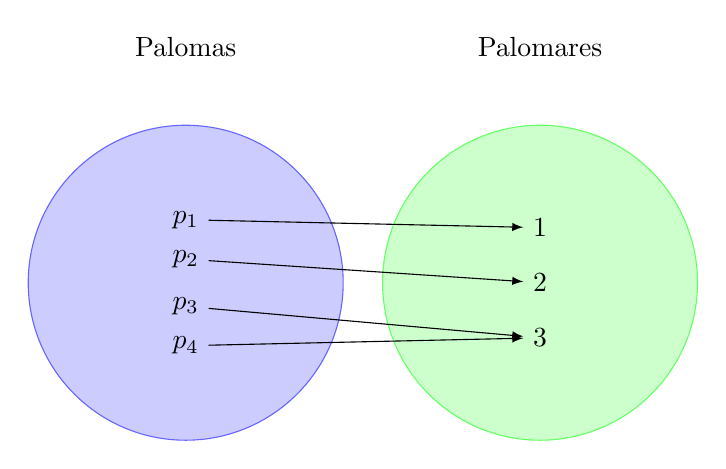
\begin{tikzpicture}
		% draw the sets
		\filldraw[fill=blue!20, draw=blue!60] (-1.5,0) circle (2cm);
		\filldraw[fill=green!20, draw=green!60] (3,0) circle (2cm);
	
	
		% the texts
		\node at (-1.5,3) {Palomas};
		\node at (3,3) {Palomares};
	
		% the circles and the arrows
		\node (x1) at (-1.5,0.8) {$p_1$};
		\node (x2) at (-1.5,0.3) {$p_2$};
		\node (x3) at (-1.5,-0.3) {$p_3$};
		\node (x4) at (-1.5,-0.8) {$p_4$};
		
		\node (y1) at (3,0.7) {$1$};
		\node (y2) at (3,0) {$2$};
		\node (y3) at (3,-0.7) {$3$};
	
		% draw the arrows
		\draw[-latex] (x1) -- (y1);
		\draw[-latex] (x2) -- (y2);
		\draw[-latex] (x3) -- (y3);
		\draw[-latex] (x4) -- (y3);
	
	\end{tikzpicture}
\caption{Ilustración del principio del palomar. El conjunto de las palomas es
mayor al del palomar, por lo tanto en al menos un palomar deben de haber dos
palomas.}
\label{palomar}
	\end{figure}

